\section{Grover on AES}

\begin{frame}{Grover on AES\footfullcite{aeslowmc}}
$N=2^k$ be the key search space. \pause $M \geq 1$ is the number of solutions. \pause The probability of finding one of the $M$ solutions after $t$ iterations is defined as 
\pause
\begin{equation*}
    p(t) = sin^2((2t+1)\theta)
\end{equation*}
\pause
which after solving for 1 gives $t\approx \frac{\pi}{4\theta} = \frac{\pi}{4} \sqrt{\frac{M}{N}}$.
\end{frame}
\begin{frame}{Key search}
Let $E_K(m) = c$ denote the encryption of message $m \in \{ 0,1\}^n$ by key $K\in \{0,1\}^k$ to ciphertext $c$. \pause Then the Grover's Oracle is defined as:

\begin{equation*}
 f(K) = 
 \begin{cases} 
      1 & E_K(m_i) = c_i  \\
      0 & else 
  \end{cases}
\end{equation*}
\pause
It is possible that multiple keys other than $K$ lead to the same ciphertext from the given plaintext. \pause Call them spurious keys.

\pause
\begin{block}{Problem}
Find the optimal number $r$ such that the probability of finding a spurious key is minimal.
\end{block}
\pause
Let $K$ be the correct key and $K'$ is spurious. Then
\pause
\begin{equation*}
    P_{K \not = K'}(E_K(m) = E_{K'}(m)) = \frac{1}{2^n}
\end{equation*}
\pause
for $r$ plaintext-ciphertext pairs, we have:
\pause
\begin{equation*}
    p = P_{K \not = K'}((E_K(m_1), \dots ,E_K(m_r) ) = (E_{K'}(m_1), \dots, E_{K'}(m_r)) )) = 2^{-nr}
\end{equation*}
\end{frame}
\begin{frame}{Key search Contd.}
    $Y$ be a binomially distributed random variable that describes the count of spurious keys for given key $K$ and $r$ plaintext-ciphertext pairs.
    \pause
    \begin{equation*}
    P(Y = y) = {2^k - 1 \choose y} p^y(1-p)^{2^k - 1- y}
\end{equation*}
\pause
Approximate this to poission distribution with $\lambda = (2^k-1)p = (2^k - 1)2^{-rn} $
\pause
\begin{equation*}
    P(Y=y) = \frac{e^{-\lambda}\lambda^k}{y!} \approx  \frac{e^{-2^{k-rn}}2^{(k-rn)y}}{y!}
\end{equation*}
\pause
$P(Y = 0) \approx e^{-2^{k-rn}}$ i.e. no spurious keys. \pause Therefore $rn > k$ or we can choose $r = \left\lceil \frac{k}{n} \right\rceil$.
\end{frame}
\begin{frame}{Parallelization of Grover}
\begin{itemize}
    \item Two ways described by \cite{tsc}\footfullcite{tsc}. Inner and outer. Multiple instances of the full Grover's algorithm are run on different machines simultaneously for a reduced number of iterations in outer parallelization.
    \pause
    \item The search space is divided into multiple disjoint subsets and each machine is assigned one subset, in case of inner parallelization.
    \pause
    \item \cite{zalka}\footfullcite{zalka} found that there is a gain of $\sqrt{S}$ in the number of iterations for $S$ parallel machines. This is inefficient as we gain only $\sqrt{S}$ factor in the depth of the quantum circuit whereas the width has become $S$ times the original. \cite{aeslowmc}\footfullcite{aeslowmc} uses inner parallelization.
\end{itemize}
\end{frame}

\begin{frame}{Why inner parallelization?}
    \begin{itemize}
        \item In outer parallelization, the probability that we find the correct key after $t$ iterations is $p_S(t) = 1 - (1-p(t))^S$.
        \pause
        \item In each machine the number of iterations will be $t_S = \frac{\pi}{4\theta\sqrt{S}}$.
        \pause
        \item General expression by using the series expansion of $sin(x)$ for larger values of $S$.
        \pause

\begin{equation*}
    p_S(t_S) = 1 - \left( 1 - \frac{\pi^2}{4S} + O\left(\frac{1}{S^2}\right) \right)^S, \sum_{y = 1}^\infty P(Y = y) = 1 - e^{-\frac{2^{k-rn}}{S}} 
\end{equation*}
\pause
\item As $S$ tends to $\infty$, the above value approaches to $1 - e^{\frac{-\pi^2}{4}} \approx 0.91$.
\pause\item This implies by just by increasing the number of parallel machines $S$, one cannot get a probability near 1 for finding the correct key.
\pause
\item For inner parallelization, the correct key exists in one of the subsets only, and with $t_S$ iterations, the machine has a near 1 probability of finding it and other machines will not find it.
\pause
\item  If spurious keys are present in a subset with the correct key not in that subset, then the spurious key can be discarded classically after the experiment. Increasing $S$ makes the above probability small. 
    \end{itemize}
\end{frame}
\begin{frame}{Quantum Circuit Design}
    Use AND gate instead of Toffoli gate. \pause The decomposition of the Toffoli gate is to 7 T gates, 8 Clifford gates with a T-depth 4 and total depth 11 \pause whereas AND gate used 4 T gates, 11 Clifford gates with T-depth 1 and total depth 8. \pause AND gate uses one ancilla qubit which is released after the operation.
    \begin{figure}[h!]
    \centering
    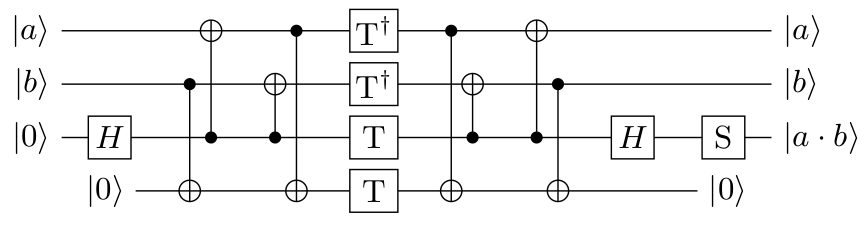
\includegraphics[width=0.6\linewidth]{aes/and.png}
    \caption{AND Gate \cite{aeslowmc}}
    \label{fig:and}
\end{figure}

\begin{figure}[h!]
    \centering
    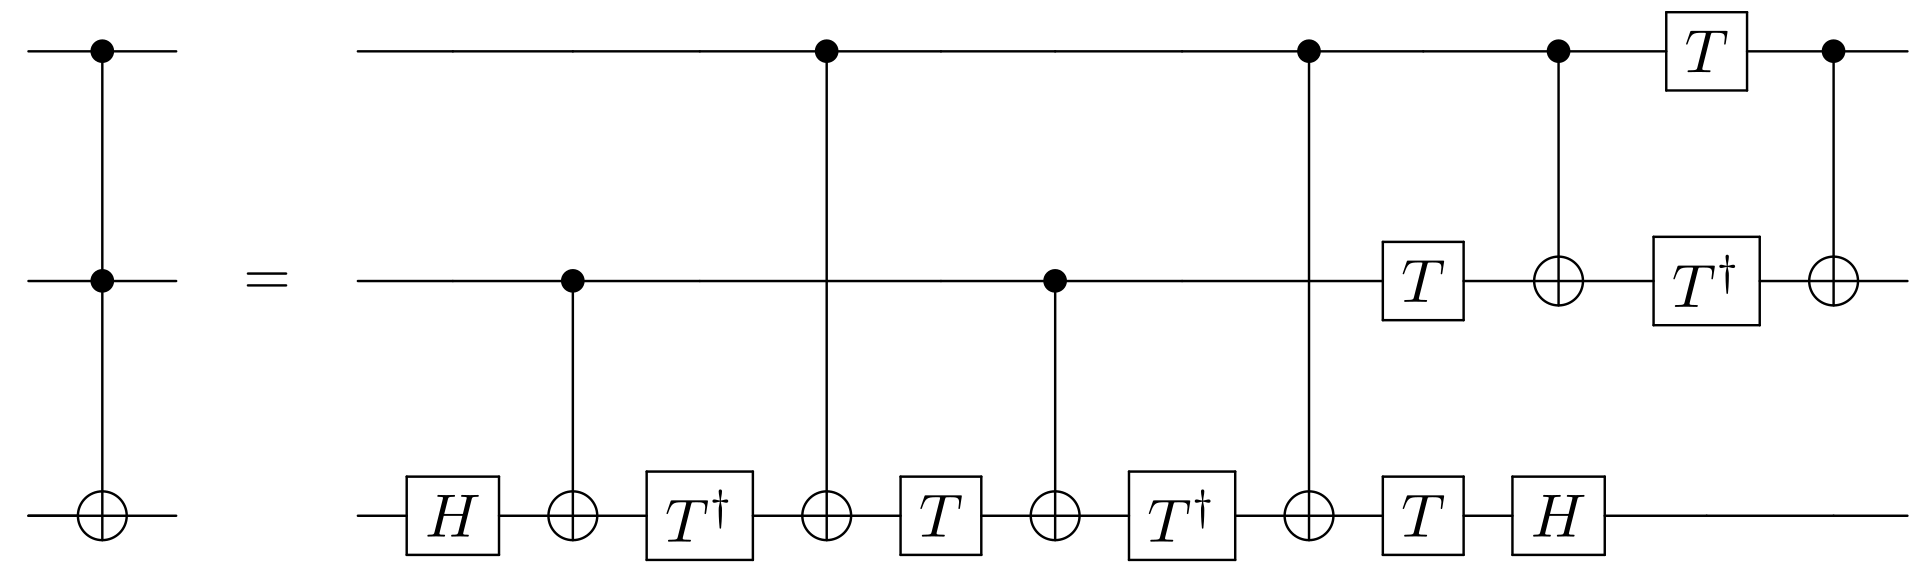
\includegraphics[width=0.6\linewidth]{aes/toffoli.png}
    \caption{Toffoli gate decomposition\cite{wiki:toff}}
    \label{fig:toff}
\end{figure}
\end{frame}
\begin{frame}{Cost Metrics}
    Depth limit $D_{max}$. \pause Two types of cost: G-cost for the total number of gates \pause and DW-cost which is the product of the depth and width of the circuit. \pause $N = 2^k$ be the key search space. \pause $S = 2^s$ is the count of parallel machines. \pause Assume that $G$ is the oracle for Grover has $G_G$ gates with $G_D$ depth using $G_W$ qubits. \pause Number of iterations for a probability $p$ i.e. $t_p = \frac{sin^{-1}(\sqrt{p})/\theta - 1}{2} \approx \frac{sin^{-1}(\sqrt{p})}{2}\sqrt{\frac{N}{S}}$. \pause Assume $sin^{-1}(\sqrt{p})/2 = c_p$.
    \pause
    \begin{equation}\label{eq:D}
    D = t_pG_D \approx c_p2^{\frac{k-s}{2}}G_D
\end{equation}
The total gate cost over all $S$ machines (G-cost) is: \pause
\begin{equation}\label{eq:gcost}
    G = t_pG_GS \approx c_p2^{\frac{k+s}{2}}G_G
\end{equation}
The total width $W = G_WS$ qubits. Therefore the DW-cost is : \pause
\begin{equation}\label{eq:DW}
    DW \approx c_p2^{\frac{s+k}{2}}G_DG_W
\end{equation}
\pause
We can see that reducing $S$ results in a reduction in DW-cost and G-cost. In case of depth constraint, attacker has to parallelize the circuit.
\end{frame}
\begin{frame}{Cost Metrics Contd.}
    We can run at most $t_{max} = D_{max}/G_D$ iterations of $G$. \pause For probablitiy $p$ of finding the correct key, we calculate $S$ i.e. $p = sin^2((2t_{max} + 1)\sqrt{\frac{S}{N}})$. This gives: \pause
    \begin{equation}\label{eq:S}
    S = \frac{(sin^{-1}(\sqrt{p}))^2N}{(2\frac{D_{max}}{G_D} + 1)^2} \approx c_p^22^k\frac{G_D^2}{D^2_{max}}
\end{equation}
\pause
\begin{equation}\label{eq:G}
    G = c_p^22^k\frac{G_DG_G}{D_{max}}
\end{equation}
\pause
\begin{equation}\label{eq:DW2}
    DW = c_p^22^k\frac{G_D^2G_W}{D_{max}}
\end{equation}
\end{frame}